\documentclass{article}
\usepackage{geometry,color,graphicx}
\usepackage{caption}
\usepackage{subcaption}
\usepackage{float}
\usepackage{amsmath}
\usepackage{empheq}

\graphicspath{ {../plots/} }

\begin{document}

\title{Project 3: Using the GNU Scientific Library and solving the Laplace equation }

\author{Gabriel Smadi\\
  Syracuse University,\\
  \texttt{gsmadi@syr.edu}}
\maketitle

\begin{abstract}
Abstract here...
\end{abstract}

\section{Introduction}

Intro here...

\section{Fraunhoffer Diffraction}

Fraunhoffer here...

\begin{figure}[H]
  \begin{center}
    \scalebox{.8}{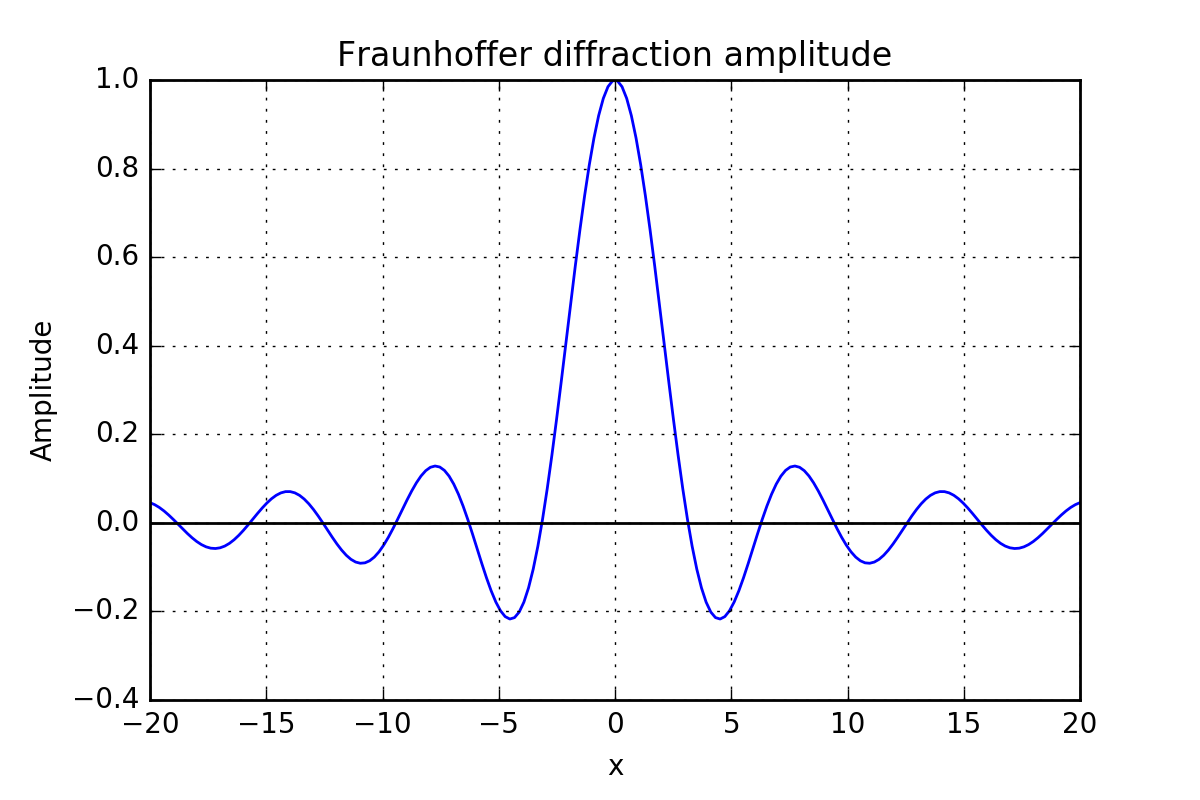
\includegraphics{fraun_amplitude}}
  \end{center}
  \caption{Convergence of errors as $h\to 0$}
  \label{fig:mag_susc}
\end{figure}

\begin{figure}[H]
  \begin{center}
    \scalebox{.8}{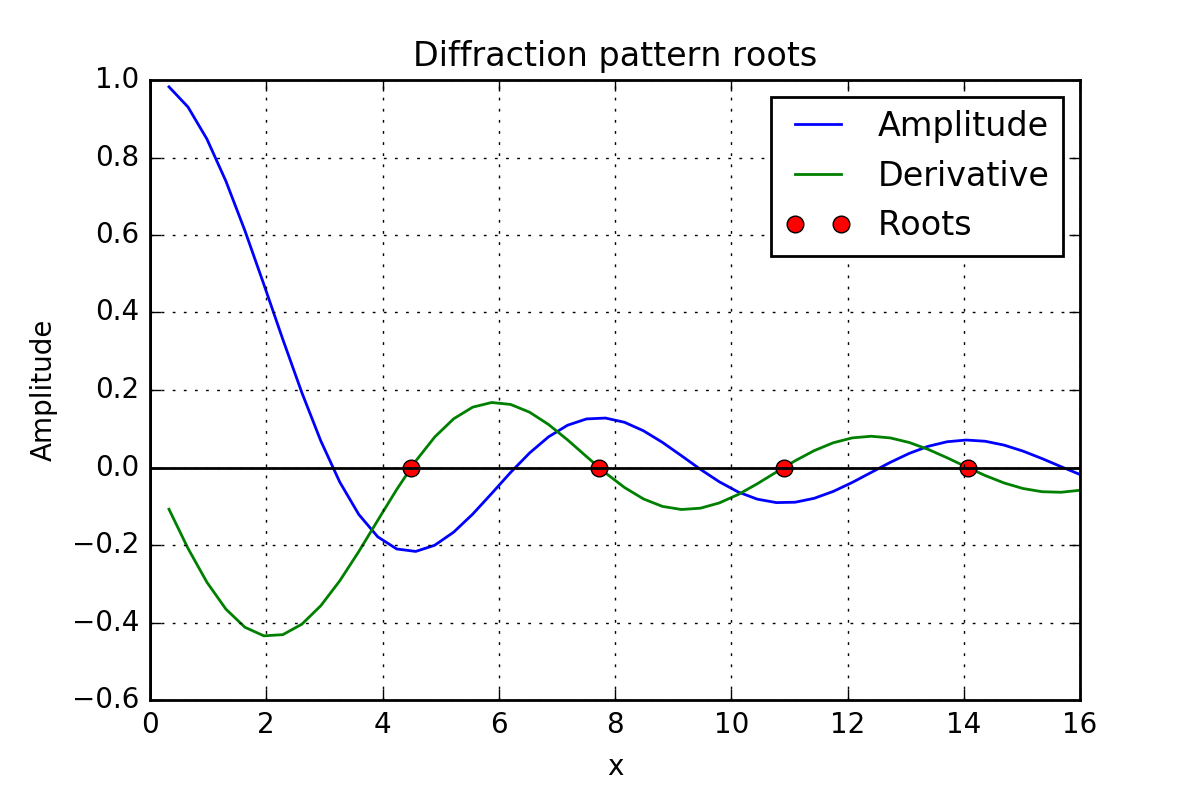
\includegraphics{fraun_root}}
  \end{center}
  \caption{Convergence of errors as $h\to 0$}
  \label{fig:mag_susc}
\end{figure}

\begin{figure}[H]
  \begin{center}
    \scalebox{.8}{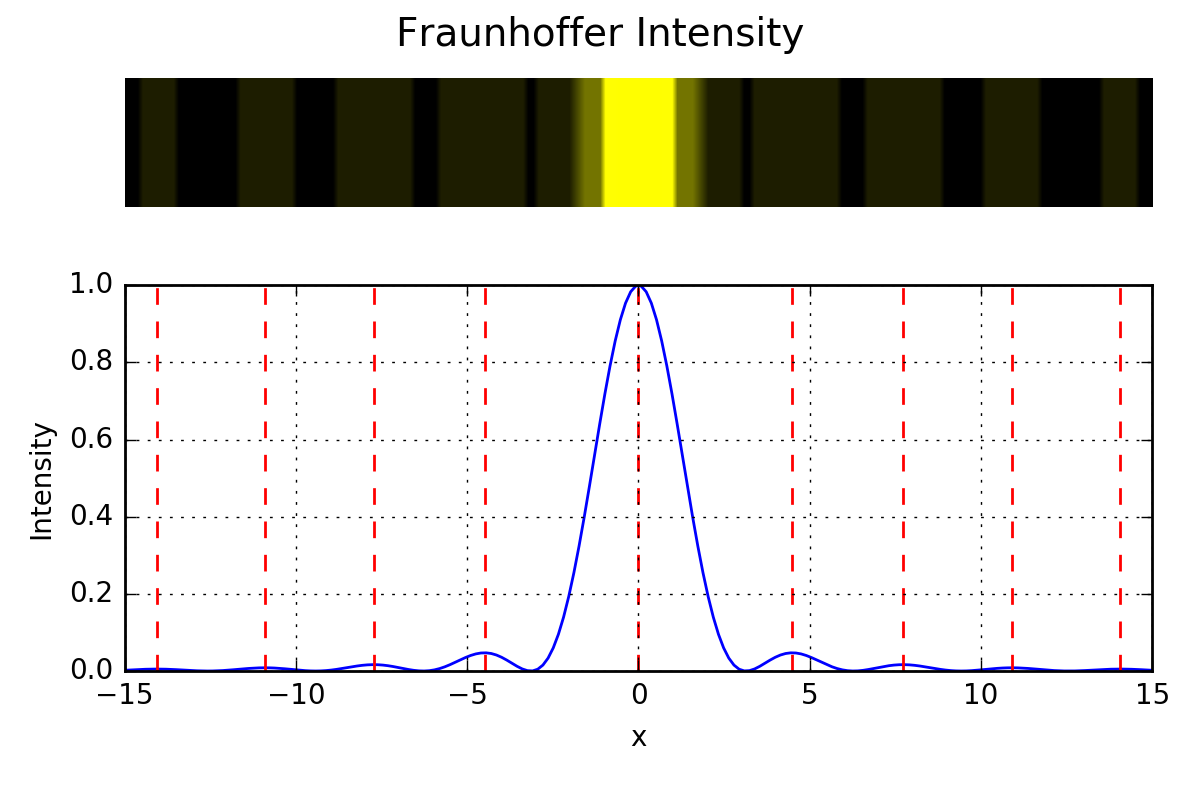
\includegraphics{fraun_int}}
  \end{center}
  \caption{Convergence of errors as $h\to 0$}
  \label{fig:mag_susc}
\end{figure}

\begin{table}[H]
  \begin{center}
    \begin{tabular}{|c|c|c|c|}
      \hline
      Iterations & Computed & Error \\
      \hline
      10 & 0.0 & 100\% \\
      \hline
      100 & 0.0 & 100\% \\
      \hline
      1000 & 1.024 & 59.8\% \\
      \hline
      10000 & 2.8672 & 12.4\% \\
      \hline
      100000 & 2.580480 & 1.2\% \\
      \hline
      1000000 & 2.56 & 0.4\% \\
      \hline
      10000000 & 2.560205 & 0.4\% \\
      \hline
      100000000 & 2.542408 & 0.3\% \\
      \hline
    \end{tabular}
  \end{center}
  \caption {Volume approximation of 10 dimensional hypersphere for several  $N$ iteration.}
  \label{tab:circle_results}
\end{table}


\section{Matrix Computations}

Matrix here...

\begin{equation}
 \label{eq:mat}
 M = \begin{bmatrix}
       1 & 2 & 3 \\[0.3em]
       2 & 2 & 3 \\[0.3em]
       3 & 3 & 3 \\[0.3em]
      \end{bmatrix}
\end{equation}

\begin{equation}
 \label{eq:mat}
 M^{-1} = \begin{bmatrix}
       -1 & 1 & 0 \\[0.3em]
       1 & -2 & 1 \\[0.3em]
       0 & 1 &  -\frac{2}{3}\\[0.3em]
      \end{bmatrix}
\end{equation}

\begin{equation}
 \label{eq:mat}
 \text{det(}M\text{)} = 3.0
\end{equation}

\begin{equation}
 \label{eq:mat}
e_{1} = \begin{bmatrix}
     0.42509 \\[0.3em]
     -0.829153 \\[0.3em]
     0.363048 \\[0.3em]
       \end{bmatrix}\text{,}\quad
e_{2} = \begin{bmatrix}
     0.765677 \\[0.3em]
     0.115485 \\[0.3em]
     -0.632774 \\[0.3em]
       \end{bmatrix}\text{,}\quad
e_{3} = \begin{bmatrix}
     0.482739 \\[0.3em]
     0.546963 \\[0.3em]
     0.683955 \\[0.3em]
       \end{bmatrix}
\end{equation}

\begin{equation}
 \label{eq:mat}
\lambda_{1} = -0.338922 \text{,}\quad
\lambda_{2} = -1.17762 \text{,}\quad
\lambda_{3} = 7.51654
\end{equation}

\begin{figure}[H]
  \begin{center}
    \scalebox{.8}{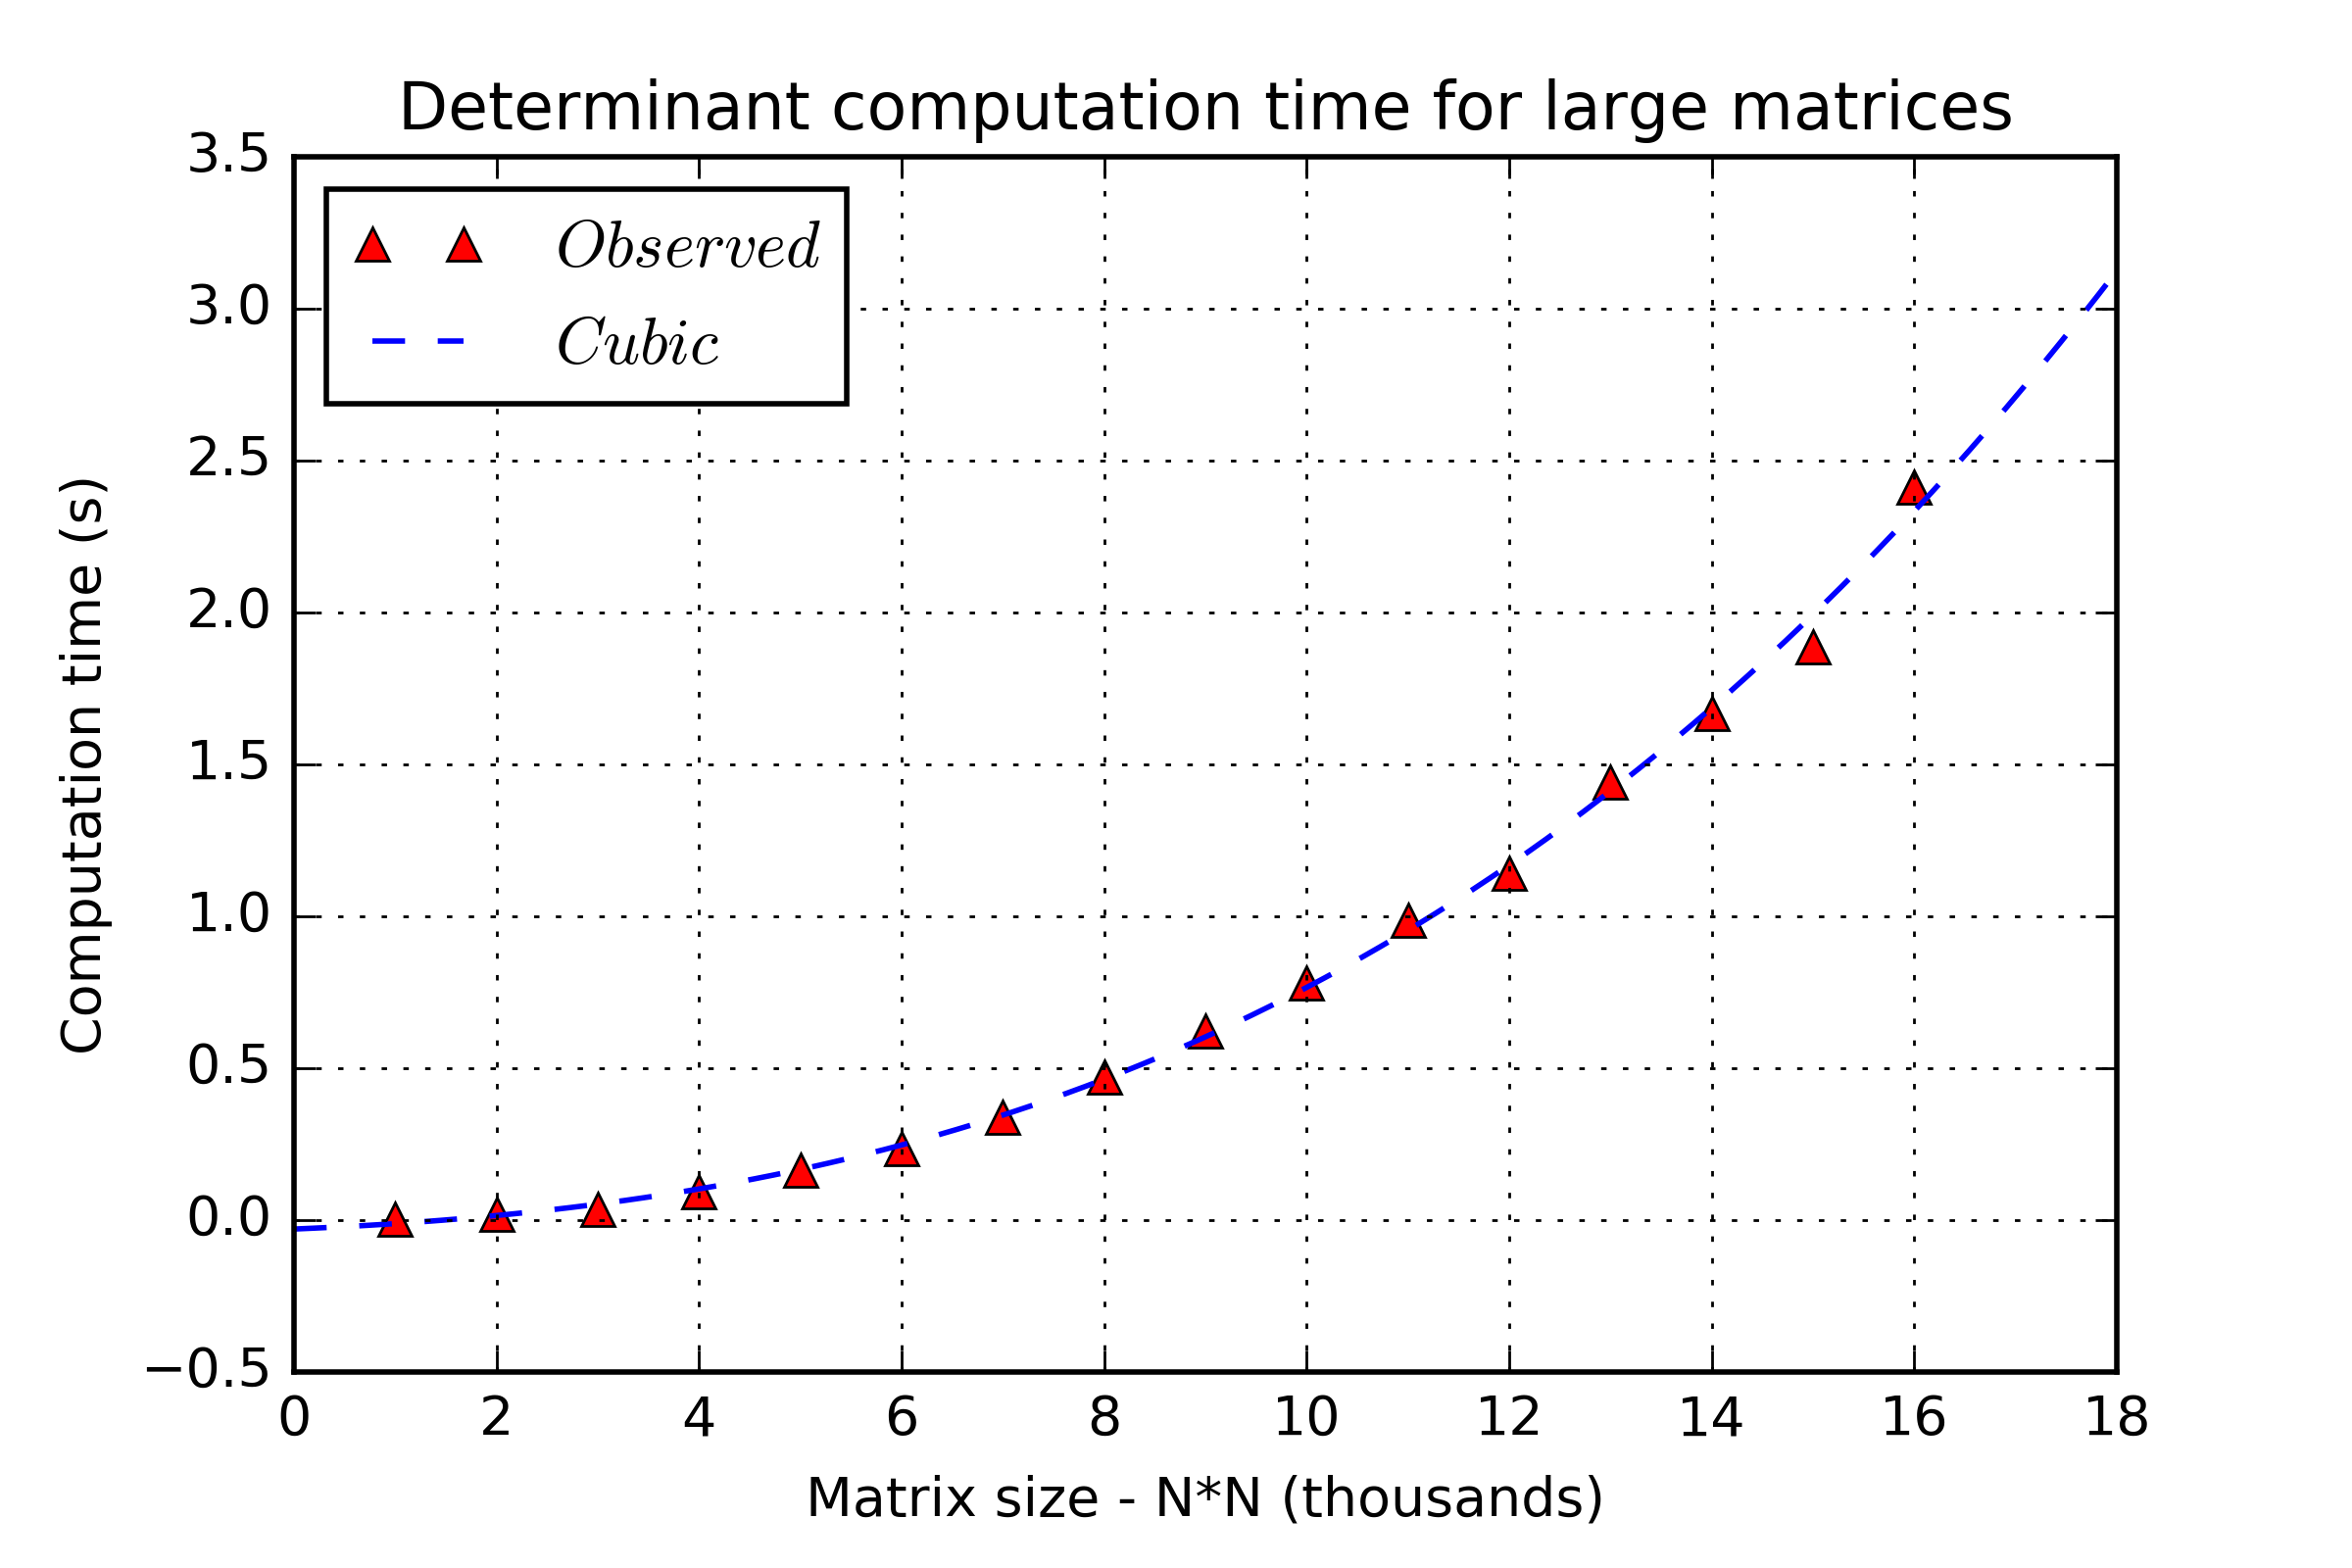
\includegraphics{det_plot}}
  \end{center}
  \caption{Convergence of errors as $h\to 0$}
  \label{fig:mag_susc}
\end{figure}


\section{Method of over-relaxation}

Relax...

\begin{figure}[H]
  \begin{center}
    \scalebox{.8}{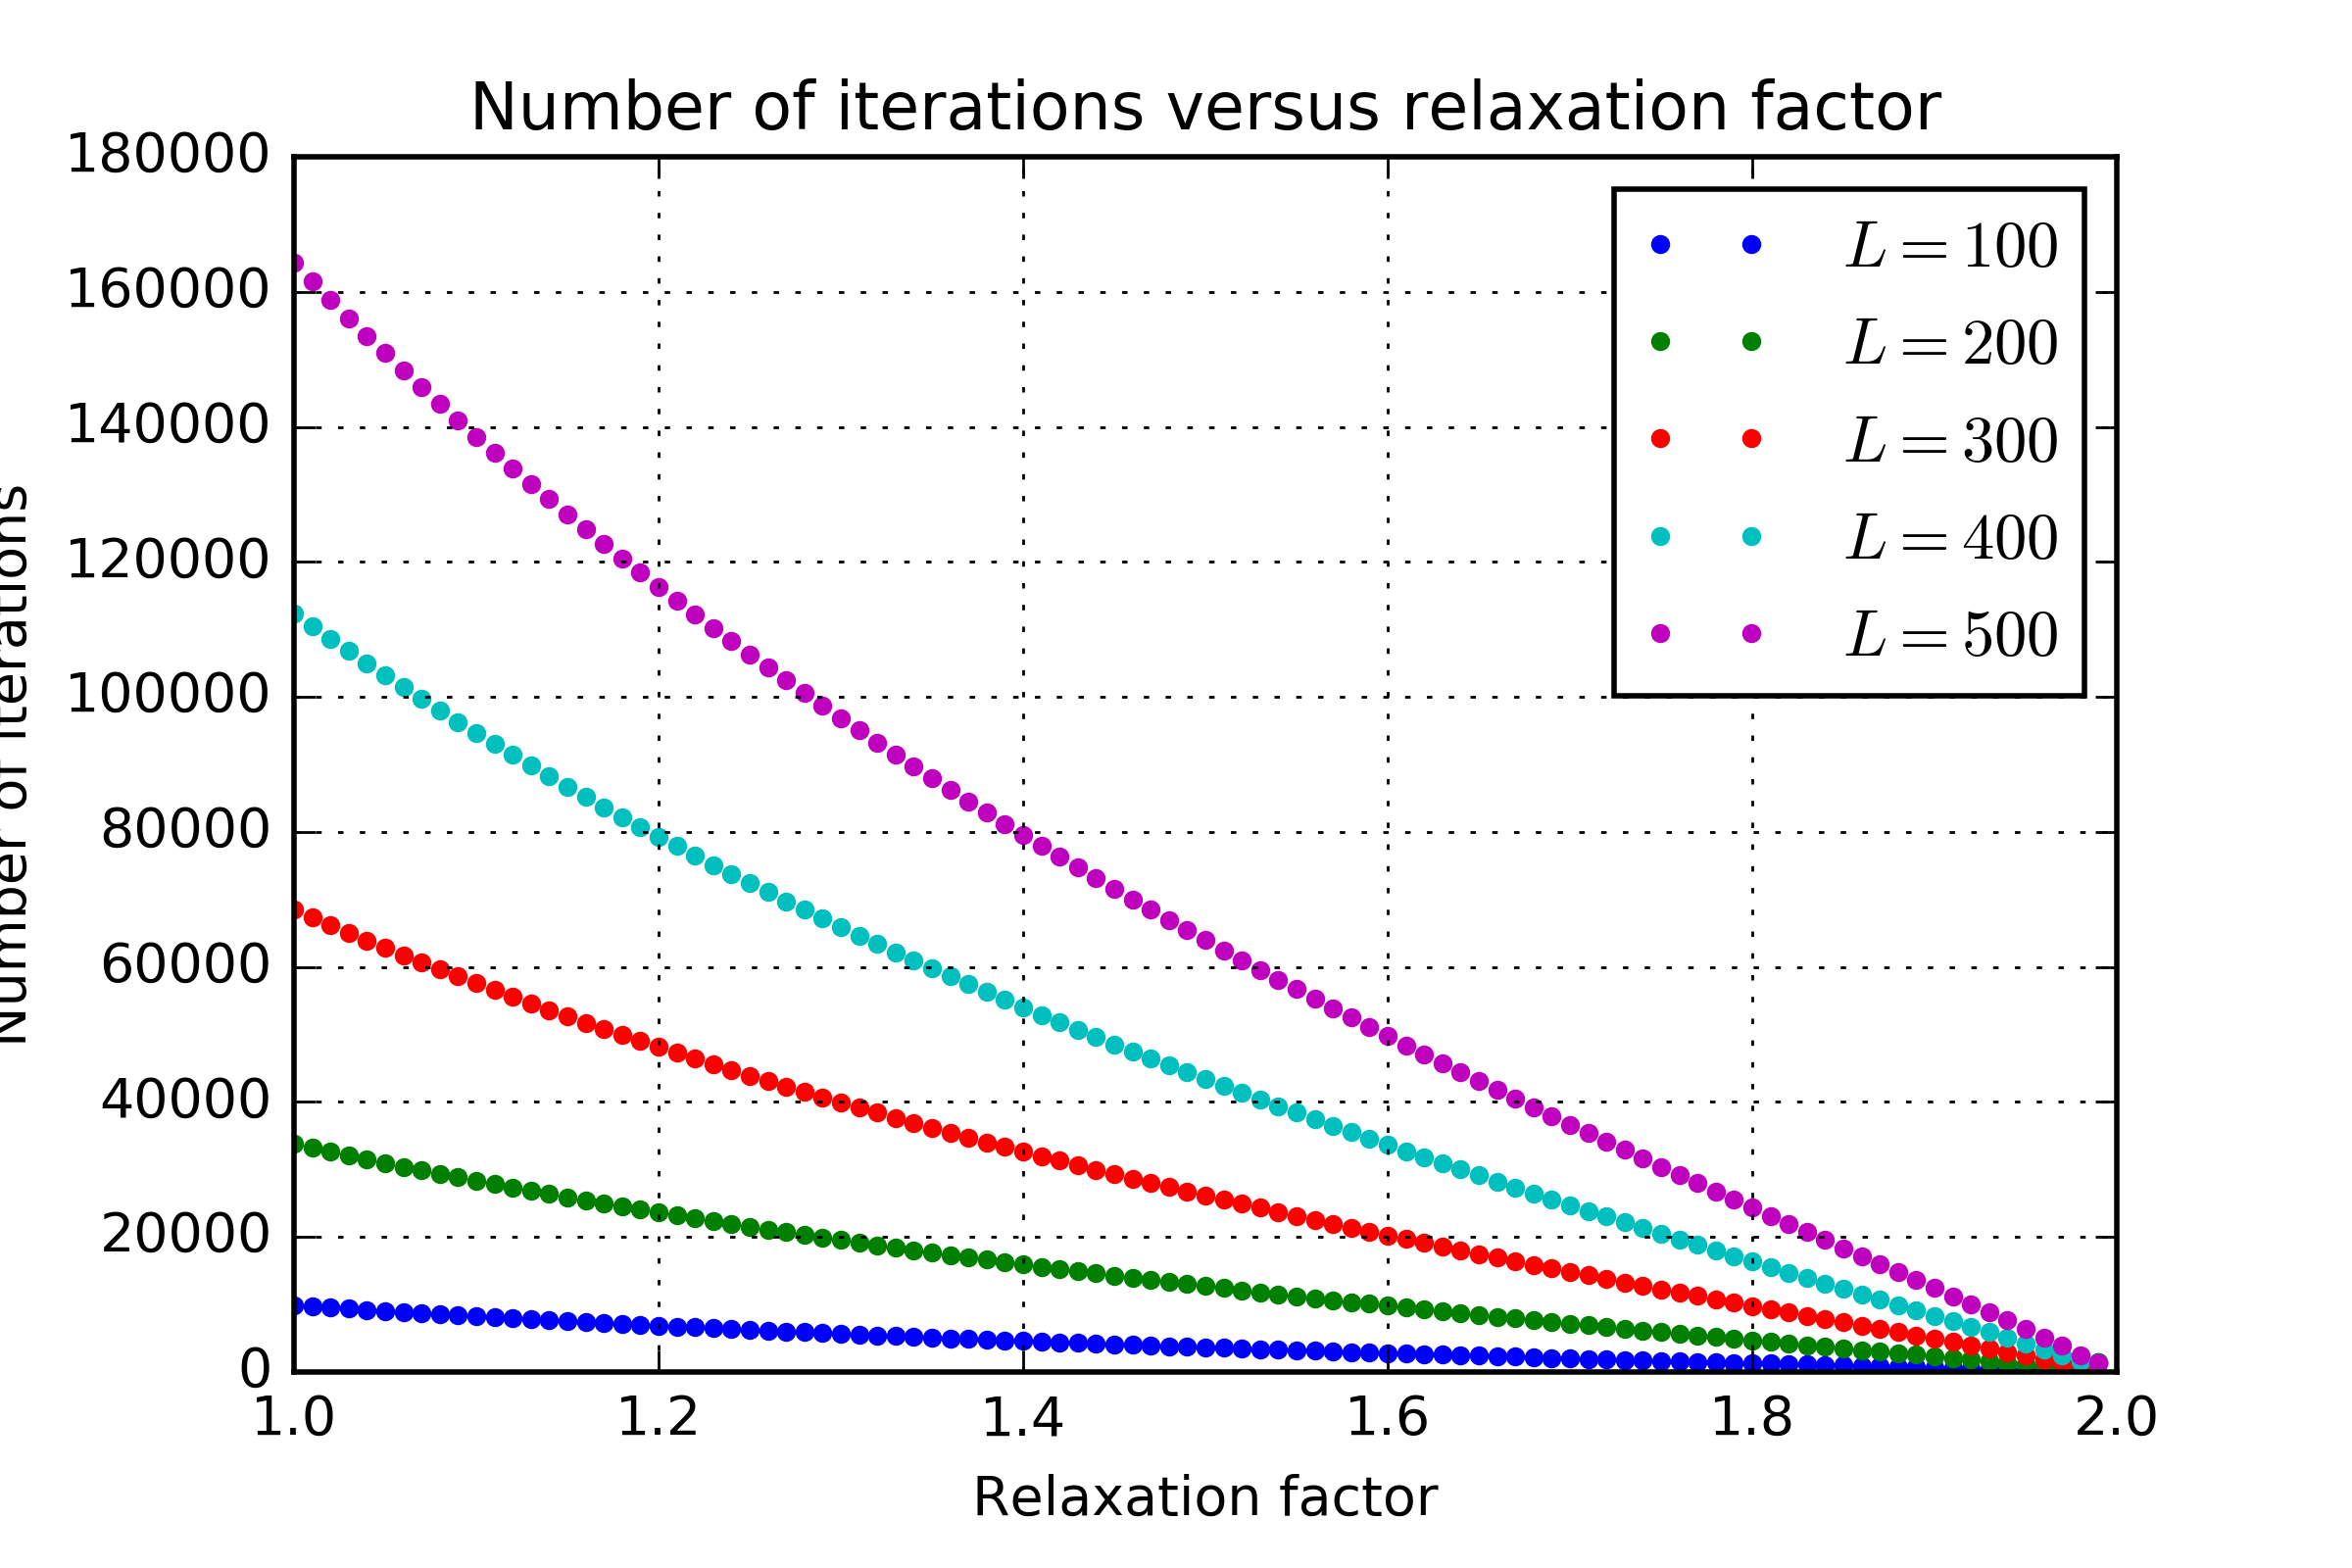
\includegraphics{iter_plot}}
  \end{center}
  \caption{Convergence of errors as $h\to 0$}
  \label{fig:mag_susc}
\end{figure}

\begin{figure}[H]
  \begin{center}
    \scalebox{.8}{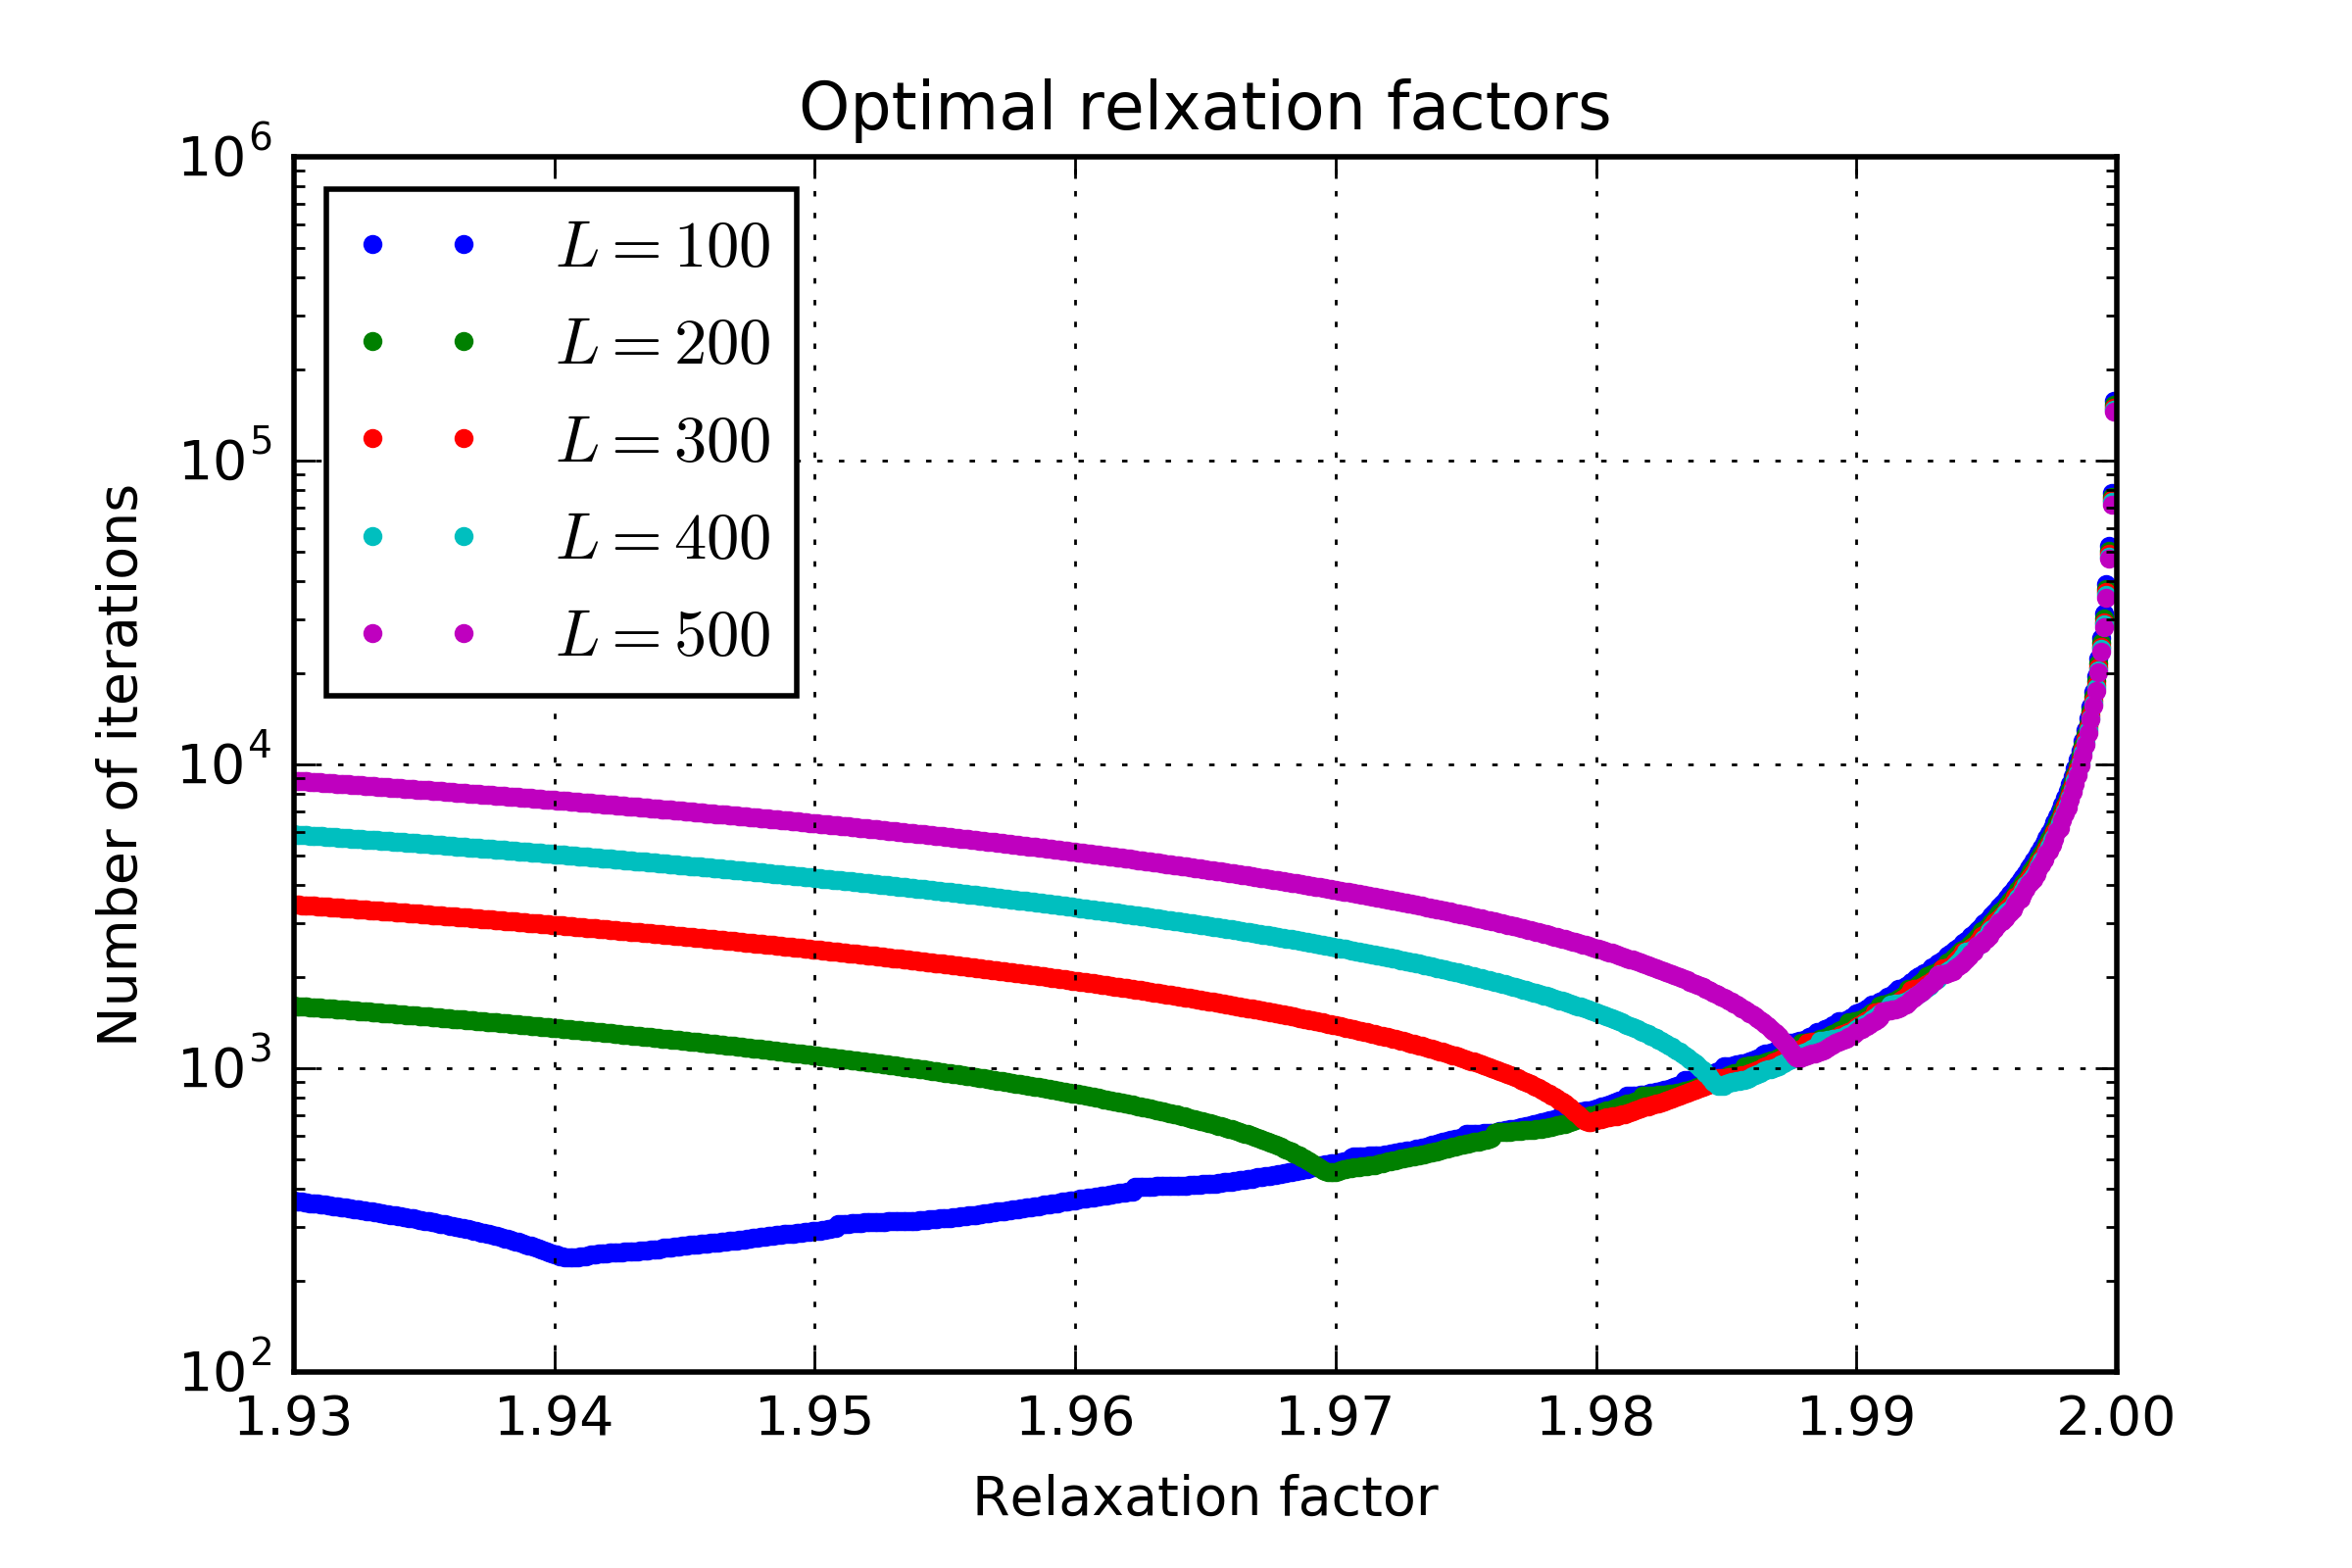
\includegraphics{iter_op_plot}}
  \end{center}
  \caption{Convergence of errors as $h\to 0$}
  \label{fig:mag_susc}
\end{figure}

\begin{figure}[H]
  \begin{center}
    \scalebox{.8}{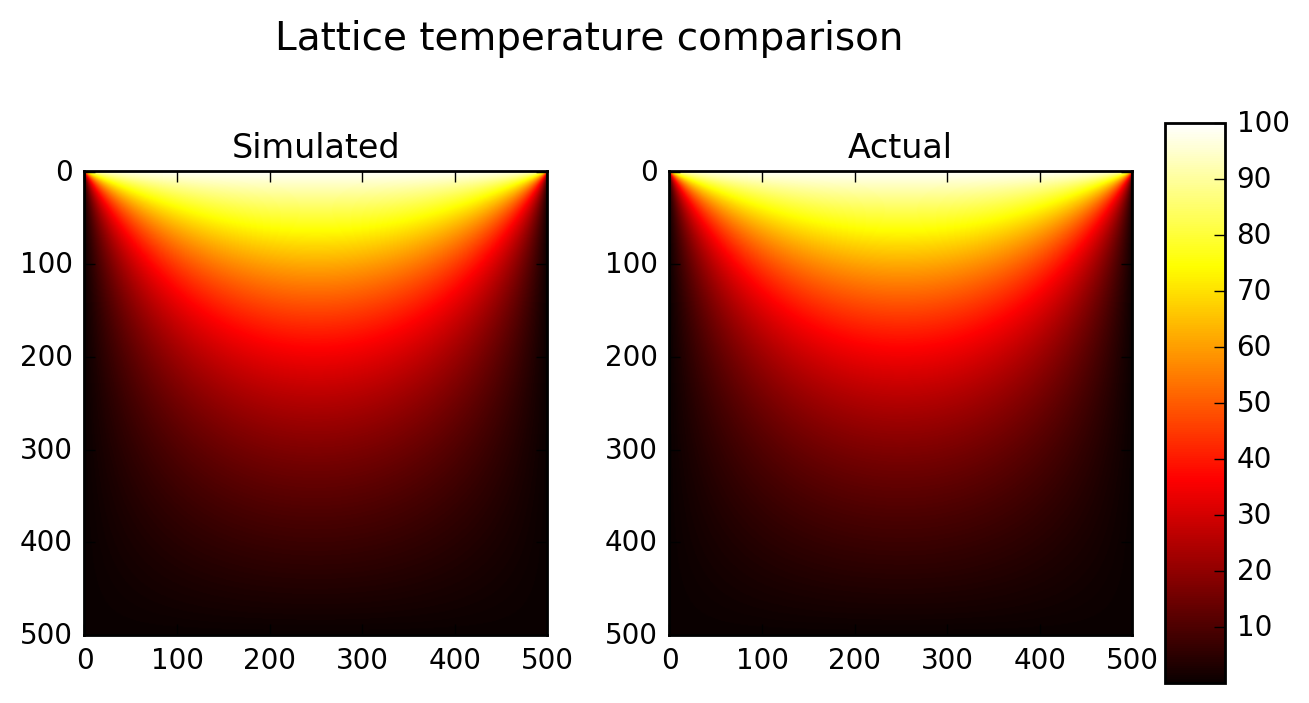
\includegraphics{temp_comp}}
  \end{center}
  \caption{Convergence of errors as $h\to 0$}
  \label{fig:mag_susc}
\end{figure}

\section{Conclusion}

Conclusion here...

\begin{thebibliography}{9}

  \bibitem{lamport94}
    Wikipedia contributors. \emph{Monte Carlo method.} Wikipedia, The Free Encyclopedia. Wikipedia, The Free Encyclopedia, 28 Mar. 2017.

  \bibitem{lamport94}
    Wikipedia contributors. "Markov chain Monte Carlo." Wikipedia, The Free Encyclopedia. Wikipedia, The Free Encyclopedia, 21 Feb. 2017.

  \bibitem{lamport94}
    Wikipedia contributors. "Square-lattice Ising model." Wikipedia, The Free Encyclopedia. Wikipedia, The Free Encyclopedia, 26 Mar. 2016.

    \bibitem{lamport94}
  	  Jacques Kotze,
  	  \emph{Introduction to Monte Carlo methods for an Ising model of ferromagnetism}.
      \tt{arXiv:cond-mat.stat-mech/0803.0217}

\end{thebibliography}
\end{document}
